\documentclass[main]{subfiles}

\begin{document}
\chapter{Electrónica}

Desde el momento que se elige realizar un trabajo de integración se corre el riesgo de trabajar con componentes que trabajan a distintos niveles de tensión. En este caso, los niveles de tensión presentes son:
\begin{itemize}
\item 11.1 V: motores
\item 5 V: alimentación de la BeagleBoard
\item 3.3 V: electrónica de los ESCs
\item 1.8 V: líneas de \emph{rx}, \emph{tx} y bus $i^2c$ de la BeagleBoard
\item La IMU puede alimentarse con cualquier voltaje menor a 16 V
\end{itemize}

Para poder integrar correctamente los diferentes componentes es necesario diseñar una placa de conversores lógicos para que lograr una correcta comunicación entre todas las partes del sistema.\\

\begin{figure}[h!]
	\centering
	\vspace{-10pt}
	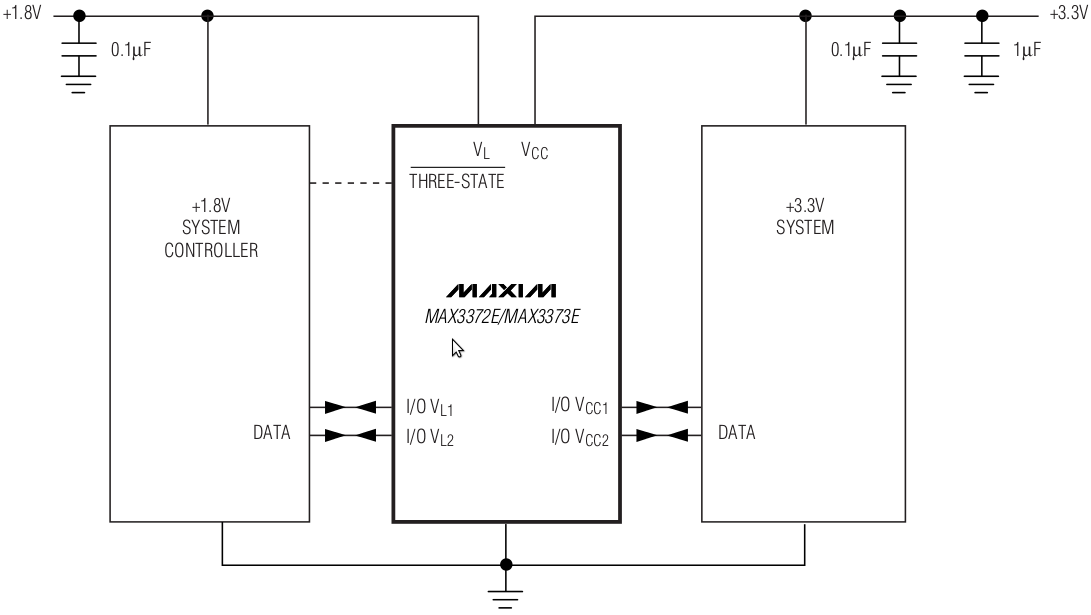
\includegraphics[width=.65\textwidth]{./pics_electronica/max.png}
	\vspace{-10pt}	
	\caption{Diagrama de conexionado del MAX3372E}
	\label{fig:max}
\end{figure}

Se elige utilizar como voltaje de entrada para la IMU el mismo voltaje que la Beagleboard, 5V.
Concretamente se debe realizar la conversión de niveles entre las líneas de bus $i^2c$ de los ESCs, que manejan 3.3V, y las líneas del bus de la Beagleboard, que manejan 1.8V y entre las líneas \emph{rx} y \emph{tx} de la IMU, que manejan 3,3V y las mismas líneas de la Beagleboard, que manejan 1.8V. Para realizar la conversión se utilizará el chip \textbf{MAX3372E}. El diagrama de conexionado se muestra en la figura \ref{fig:max}, tomada de la hoja de datos del dispositivo mencionado.

Es importante destacar la necesidad de la bidireccionalidad de las líneas del bus $i^2c$ ya que tanto el amo como los esclavos deben ser capaces de realizar cambios sobre la misma. Como se puede ver en la figura antes mencionada, el chip posee 2 líneas bidireccionales que serán utilizadas para las líneas \emph{SDA} y \emph{SCL} del bus $i^2c$. Para las líneas de transmisión serial es suficiente con un par de líneas unidireccionales, pero de todas formas se decide utilizar el mismo chip por razones de simplicidad.\\

La placa de conversión de niveles lógicos será alimentada con las líneas de 5V y 1.8V presentes en la cabecera de expansión de la Beagleboard. Para generar los 3.3V necesarios para alimentar los 2 chips MAX3372E se utiliza el regulador de tensión \textbf{LD33V}. A su vez la placa otorgará la posibilidad de alimentarla con la misma batería que utilizan los motores, es decir, alimentarla con 11.1V. En este caso se utiliza el regulador de tensión \textbf{L7805CV} para generar una línea de 5V a partir de la entrada de 11.1V, que será utilizada para alimentar la Beagleboard. De esta manera se logra eliminar una de las baterías del sistema, la BeagleJuice, logrando reducir aproximadamente 130g la masa del sistema.\\

\begin{figure}[h!]
	\centering
	\vspace{-12pt}
	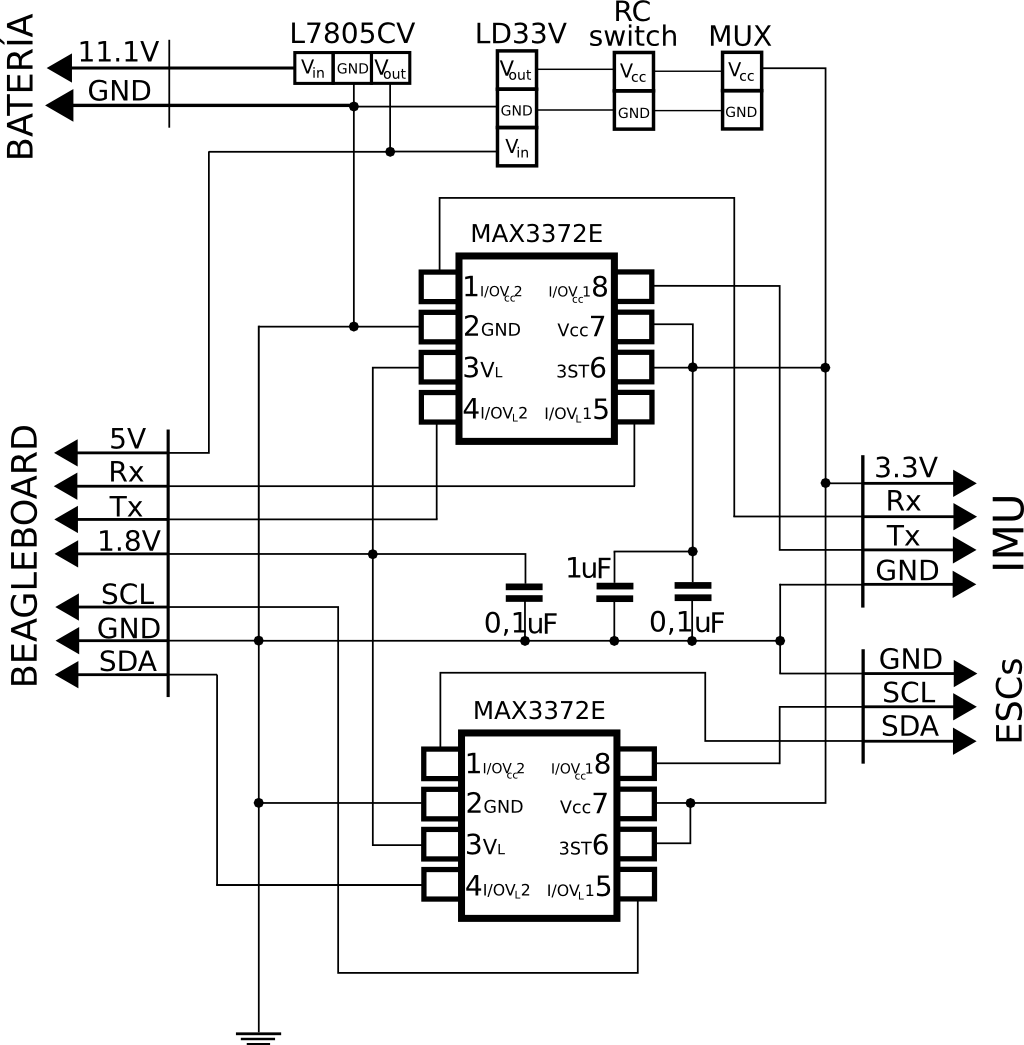
\includegraphics[width=.75\textwidth]{./pics_electronica/esquema_plaquita.png}
	\caption{Placa conversores lógicos y switcheo}
	\label{fig:plaquita}
\end{figure}

Por último se incluye en la misma un par de pines necesarios para alimentar el \emph{switch RC} y el \emph{multiplexor} necesarios para realizar la conmutación entre el mando automático y el manual, explicado en el capítulo \ref{chap:anexo_switcheo}.\\

El diseño final de la placa es el mostrado en la figura \ref{fig:plaquita}.

\end{document}